\section{Design}
During our brainstorm sessions it quickly became clear that we needed a policy engine that was flexible. With inspiration from other building management systems (see related work) and looking at the web service we had to communicate with, we came up with the concept of policies that consist of rules.

\subsection{Policy}
A policy in our project is defined as a set of rules that can be activated in a given setting.

\subsection{Rules}
It's in the rules that the power of our engine lies. We have striven to create a model for rules that are flexible and yet simple. A rule is defined as a "`IF THEN ELSE"' statement, that can contain expressions that supports the logical operators of AND, OR and the relational operators LESS THAN, GREATER THAN, EQUALS, NOT. 

Using this setup allows us to construct rules in a matter similar to other DSL languages such as SQL. Below is an example from a rule we can construct with our engine:
\\
\\
\\
\\
\\
\begin{lstlisting}[language=json,firstnumber=1]
{"statements":[

// Define IF statement
{"type":"IfStatement","data": {"conditionalExpressions":[{"prefixOperator":"AND","aValue":
	{"type":"IntValue","data":{"theValue":10}},"operator":"EQUALS","sensorId":"ROOM1.TEMPERATURE"}],

// Define THEN statement	
	"thenStatements":[{"type":"SetStatement","data":{"aValue":
	{"type":"BooleanValue","data":{"theValue":true}},"sensorID":"ROOM1.HEATER"}}],

// Define ELSE statement
	"elseStatements":[{"type":"SetStatement","data":
	{"aValue":{"type":"BooleanValue","data":{"theValue":true}},"sensorID":"ROOM1.BLINDS"}}]}}]}
\end{lstlisting}

What happens in this example is ...

\subsection{High level design}

\begin{figure}[t]
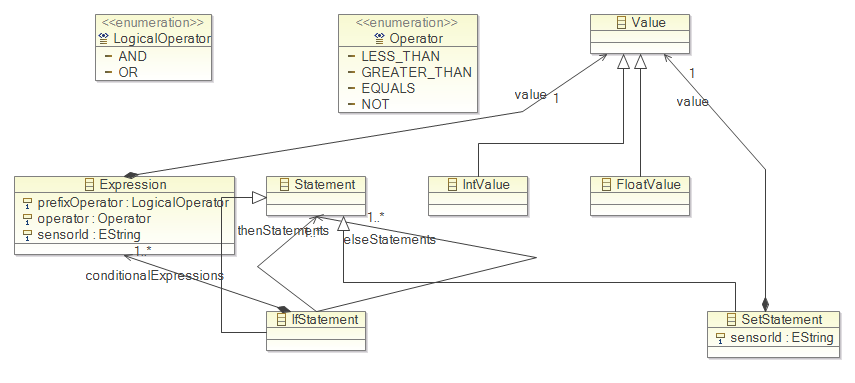
\includegraphics[width=1.00\columnwidth]{model.png}
\caption{Model}
\end{figure}


\subsection{Limitations}
... Alternatives?